% CSE731 Software Testing -- Mid-term Project Report
% Compile with: tectonic report.tex  (run from the project root)
\documentclass[11pt,a4paper]{article}
\usepackage[T1]{fontenc}
\usepackage[utf8]{inputenc}
\IfFileExists{lmodern.sty}{\usepackage{lmodern}}{}
\usepackage[margin=2.2cm]{geometry}
\usepackage{booktabs,tabularx,array,float,caption,amsmath}
\usepackage{xcolor,listings}
\usepackage{tikz}
\usetikzlibrary{arrows.meta,positioning}
\usepackage[colorlinks=true,linkcolor=black,urlcolor=blue!50!black]{hyperref}
\emergencystretch=3em
\setlength{\parskip}{4pt}
\captionsetup{font=small,labelfont=bf}

\definecolor{codebg}{RGB}{247,247,249}
\lstdefinestyle{plain}{basicstyle=\ttfamily\footnotesize,backgroundcolor=\color{codebg},
  frame=single,rulecolor=\color{gray!40},breaklines=true,columns=fullflexible,
  keepspaces=true,showstringspaces=false,captionpos=b}
\lstdefinestyle{py}{style=plain,language=Python,keywordstyle=\color{blue!60!black}\bfseries,
  stringstyle=\color{red!60!black},commentstyle=\color{green!40!black}\itshape}
\lstset{style=plain}

\newcommand{\artifact}[2]{\IfFileExists{#1}%
  {\lstinputlisting[style=py,caption={#2}]{#1}}%
  {\par\noindent\fcolorbox{red!70!black}{red!4}{\parbox{\dimexpr\linewidth-2\fboxsep-2\fboxrule}{\small
   \textbf{Missing:} \texttt{\detokenize{#1}}}}\par\medskip}}

\begin{document}

\begin{center}
{\large\bfseries International Institute of Information Technology Bangalore}\\[2pt]
CSE731: Software Testing \;--\; Mid-term Project, Term I (2026--27)\\[10pt]
{\LARGE\bfseries Agentic AI Pipeline for Coverage-Directed Unit Test Generation}\\[10pt]
\begin{tabular}{ll}
Sanyam Verma & IMT2023040\\
Gautam Kappagal & IMT2023082
\end{tabular}
\end{center}

\noindent\textbf{Testing requirement pursued:} (1) user-specified coverage criterion --
statement coverage and branch coverage, target 100\%.

% ======================================================================
\section{Pipeline, Dataset and Test-Generator Functionality}

\textbf{Dataset.} MBPP (\texttt{google-research-datasets/mbpp}), \texttt{train} split,
five problems (task IDs 601, 602, 604, 605$\times$2). Task ID 603 (``lucid number'')
was skipped because all tested free models consistently returned syntactically invalid
Python for that prompt; the pipeline's \texttt{--skip-mbpp-ids} flag substituted the
next available problem. MBPP 605 was run twice independently (different random
seeds / model assignments), providing a comparison of two generated implementations of
the same specification. Only the natural-language task is given to the pipeline; MBPP's
reference code and tests are stored alongside for traceability.

\begin{table}[H]
\centering\small
\begin{tabularx}{\linewidth}{c X}
\toprule
MBPP ID & Task\\
\midrule
601 & Write a function to find the longest chain which can be formed from the given set of pairs.\\
602 & Write a python function to find the first repeated character in a given string.\\
604 & Write a function to reverse words in a given string.\\
605 (trial A) & Write a function to check if the given integer is a prime number.\\
605 (trial B) & Write a function to check if the given integer is a prime number.\\
\bottomrule
\end{tabularx}
\caption{MBPP problems used (five pipeline runs).}
\end{table}

\textbf{Agents.} The pipeline is plain Python (one class per agent, a loop in
\texttt{pipeline.py}, direct HTTPS calls to OpenRouter); no RAG, no agent framework
and no chain-of-thought prompting is used.
\begin{enumerate}
  \item \textbf{Code Generator Agent} (LLM): MBPP task $\rightarrow$ \texttt{solution.py}.
  \item \textbf{Test Generator Agent} (LLM): task + generated code + coverage criterion
        $\rightarrow$ \texttt{test\_solution.py} (Python \texttt{unittest}).
  \item \textbf{Test Executor Agent} (deterministic): runs the suite under
        \texttt{coverage.py} in branch mode and returns the verdict
        (PASS/FAIL/TIMEOUT), statement \%, branch \% and the uncovered lines/branches.
        Execution and coverage are measured by tools rather than an LLM so the verdict cannot be hallucinated.
\end{enumerate}

\begin{figure}[H]
\centering
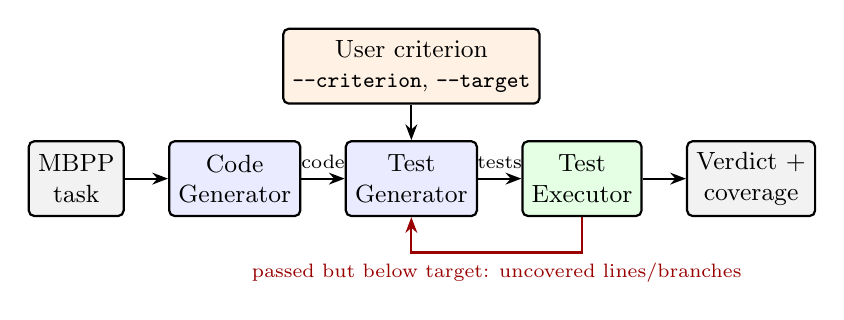
\begin{tikzpicture}[node distance=0.55cm and 0.55cm,
  b/.style={draw,rounded corners=2pt,thick,align=center,font=\small,minimum height=0.95cm},
  a/.style={-{Stealth[length=2mm]},thick}]
  \node[b,fill=gray!10] (d) {MBPP\\task};
  \node[b,fill=blue!8,right=of d] (c) {Code\\Generator};
  \node[b,fill=blue!8,right=of c] (t) {Test\\Generator};
  \node[b,fill=green!10,right=of t] (e) {Test\\Executor};
  \node[b,fill=gray!10,right=of e] (o) {Verdict +\\coverage};
  \node[b,fill=orange!10,above=0.45cm of t] (u) {User criterion\\\footnotesize\texttt{--criterion}, \texttt{--target}};
  \draw[a] (d)--(c); \draw[a] (c)-- node[above,font=\scriptsize]{code}(t);
  \draw[a] (t)-- node[above,font=\scriptsize]{tests}(e); \draw[a] (e)--(o);
  \draw[a] (u)--(t);
  \draw[a,red!60!black] (e.south) -- ++(0,-0.45) -| node[pos=0.25,below,font=\scriptsize]{passed but below target: uncovered lines/branches} (t.south);
\end{tikzpicture}
\caption{Pipeline. Blue: LLM agents; green: deterministic executor agent.}
\end{figure}

\textbf{Test-generator functionality.} The user selects the criterion
(\texttt{statement+branch} (default), \texttt{statement} or \texttt{branch}) and a target.
The prompt asks for representative, boundary and edge inputs, both outcomes of every
conditional, and zero/one-or-more loop iterations. Coverage is computed as
\[
\text{Stmt\%}=\frac{\text{statements}-\text{missing}}{\text{statements}}\times100,\qquad
\text{Branch\%}=\frac{\text{covered branches}}{\text{total branches}}\times100 .
\]
If a suite passes but misses the target, the executor's list of uncovered statements
and branch outcomes is sent back to the Test Generator to extend the suite (at most 2
rounds). Failing suites are not sent back, since a failure may reveal a real defect in
the code. Generated output is rejected unless it parses (\texttt{ast.parse}), and test
modules must use \texttt{unittest} and contain a \texttt{test\_} method. On a
validation failure the agent automatically retries with the next available free model,
excluding the model that returned invalid output.

% ======================================================================
\section{Prompts and Settings}

Each agent fills a fixed template and sends it as a single \texttt{user} message (no
system message, no history). The user input is the MBPP slice (\texttt{-n}) and the
testing requirement (\texttt{--criterion}, \texttt{--target}).

\begin{lstlisting}[caption={Code Generator prompt.}]
You are the Code Generator Agent in an automated software-testing experiment.

Programming problem:
{task}

Generate a correct Python implementation for the problem.

Strict output rules:
- Return ONLY executable Python source code.
- Do not use Markdown code fences.
- Do not include explanations.
- Do not include JSON.
- Do not include safety classifications.
- Do not include analysis.
- Define the function(s) required by the problem.
- Keep the implementation concise and self-contained.
\end{lstlisting}

\begin{lstlisting}[caption={Test Generator prompt. Item 10 depends on the chosen criterion; for \texttt{statement+branch} it is ``Aim for high statement and branch coverage.''}]
You are the Test Generator Agent in an AI-assisted unit-testing pipeline.

Programming problem:
{task}

Generated Python implementation:
{implementation}

Create a complete Python unittest module named test_solution.py.

Test-design requirements:
1. Use Python's built-in unittest framework.
2. Import the function(s) from solution.py.
3. Include normal/representative cases.
4. Include boundary cases where meaningful.
5. Include edge cases such as empty, singleton, negative,
   duplicate, or unusual inputs when applicable.
6. For each important conditional, exercise both outcomes.
7. For loops, exercise zero iterations and one-or-more iterations
   when meaningful.
8. Use strong assertions with expected outputs.
9. Do not test implementation details that are irrelevant to the
   problem specification.
10. {criterion_text}

Strict output rules:
- Return ONLY executable Python source code.
- Do not use Markdown code fences.
- Do not include explanations.
- Do not include JSON.
- Do not include safety classifications.
\end{lstlisting}

The coverage-feedback prompt repeats the task, the code with line numbers and the
current tests, adds ``Statements never executed: \ldots'' and ``Branch outcomes never
taken: \ldots'' from the executor, and asks for the complete updated module.

\begin{table}[H]
\centering\small
\begin{tabularx}{\linewidth}{l X}
\toprule
Parameter & Value\\
\midrule
LLM provider & OpenRouter free models (auto-discovered; excluded per-call on validation failure)\\
Models used & \texttt{nvidia/nemotron-3.5-lightning:free}, \texttt{qwen/qwen3.8-27b:free},\\
            & \texttt{nvidia/nemotron-3-ultra-550b-a55b:free}, \texttt{nvidia/nemotron-3-nano-omni-30b-a3b-reasoning:free}\\
Temperature & 0.2 (all LLM calls)\\
\texttt{max\_tokens} & 1500 (code), 2500 (tests)\\
Other sampling parameters & provider defaults\\
HTTP timeout & 10\,s connect, 60\,s read\\
Test framework / coverage & \texttt{unittest}; \texttt{coverage run --branch --source=solution}\\
Executor timeout & 180\,s per suite\\
Criterion / target & statement + branch, 100\%\\
\bottomrule
\end{tabularx}
\caption{Pipeline settings.}
\end{table}

% ======================================================================
\section{Format of Code, Tests and Verdict}

\textbf{Code:} \texttt{generated/problem\_N/solution.py}, a plain Python module with the
required function(s). \textbf{Tests:} \texttt{generated/problem\_N/test\_solution.py}, a
\texttt{unittest.TestCase} class with one \texttt{test\_*} method per scenario using
\texttt{assertEqual}/\texttt{assertTrue}/\ldots\ with explicit expected values.
\textbf{Verdict:} a JSON record saved in \texttt{experiment.json}:
\begin{lstlisting}
{ "verdict": "PASS", "passed": true, "tests_run": 16,
  "statement_coverage": 100.0, "branch_coverage": 100.0,
  "missing_lines": [], "missing_branches": [],
  "execution_time_seconds": 0.1, "stderr": "Ran 16 tests in 0.001s  OK" }
\end{lstlisting}

\subsection*{Generated code and test cases}
\artifact{generated/problem_1/solution.py}{MBPP 601 -- generated code}
\artifact{generated/problem_1/test_solution.py}{MBPP 601 -- generated tests}
\artifact{generated/problem_2/solution.py}{MBPP 602 -- generated code}
\artifact{generated/problem_2/test_solution.py}{MBPP 602 -- generated tests}
\artifact{generated/problem_3/solution.py}{MBPP 604 -- generated code}
\artifact{generated/problem_3/test_solution.py}{MBPP 604 -- generated tests}
\artifact{generated/problem_4/solution.py}{MBPP 605 trial A -- generated code}
\artifact{generated/problem_4/test_solution.py}{MBPP 605 trial A -- generated tests}
\artifact{generated/problem_5/solution.py}{MBPP 605 trial B -- generated code}
\artifact{generated/problem_5/test_solution.py}{MBPP 605 trial B -- generated tests}

% ======================================================================
\section{Execution Results}

\begin{table}[H]
\centering\small
\begin{tabular}{c c c c c r}
\toprule
MBPP ID & Tests generated & Verdict & Statement cov. & Branch cov. & Runtime (s)\\
\midrule
601         &  7 & PASS & 100\% & 100\% & 281.0\\
602         & 16 & PASS & 100\% & 100\% &  69.1\\
604         & 14 & PASS & 100\% & 100\% &  71.9\\
605 (A)     &  8 & PASS & 100\% & 100\% & 262.7\\
605 (B)     & 11 & PASS & 100\% & 100\% & 242.1\\
\midrule
\textbf{Total} & \textbf{56} & \textbf{5/5} & \textbf{100\%} & \textbf{100\%} & \textbf{926.8}\\
\bottomrule
\end{tabular}
\caption{Results of the Test Generator and Test Executor agents. Runtime includes LLM latency.}
\end{table}

All five suites met the criterion on the first attempt, so no coverage-feedback round
was needed. Test execution itself took under a second per problem; nearly all runtime
was LLM latency on free-tier models (e.g.\ MBPP 601: 56.5\,s code generation,
224.0\,s test generation, $<$0.1\,s execution).

The two independent runs of MBPP 605 generated structurally different implementations
(trial A uses the $6k\pm1$ divisibility optimisation; trial B uses a simple odd-step
loop) and different test suites (8 vs.\ 11 methods), both achieving 100\% statement
and branch coverage.

\textbf{Limitations.} 100\% statement and branch coverage shows every statement and
decision outcome was executed, not that the code is correct: the tests are written
from the generated code, so a misunderstanding shared by both would still PASS. Task ID
603 (``lucid number'') was skipped because free models consistently returned
syntactically invalid Python for it, suggesting the task description is ambiguous or
too obscure for small free-tier models. Running MBPP's reference tests or mutation
testing would give an independent correctness signal.

% ======================================================================
\section{Individual Contributions}

\begin{table}[H]
\centering\small
\begin{tabularx}{\linewidth}{l X}
\toprule
Member & Contribution\\
\midrule
Sanyam Verma (IMT2023040) &
Selected the testing goal (coverage criterion) and dataset; built the Code Generator and
Test Generator agents and the OpenRouter client; designed the test-generation prompt
(boundary/edge cases, both outcomes of each decision, loop iterations) and the
coverage-feedback loop; output validation of generated code and tests; per-call model
exclusion on validation failure.\\
Gautam Kappagal (IMT2023082) &
Built the Test Executor agent: running suites with \texttt{unittest} and
\texttt{coverage.py}, statement/branch coverage computation, PASS/FAIL/TIMEOUT verdicts;
pipeline orchestration and result logging; ran the experiment, analysed the coverage
results and limitations, and wrote the report.\\
\bottomrule
\end{tabularx}
\end{table}

\end{document}
